\subsection{Cosmogenic Activation in the Liquid Xenon}
\label{secCosmogenicActivationLXe}

%The cosmogenic activation of xenon, has not been measured. However, with the increase of the sensitivity of the 

\begin{table}[!t]
\centering
\caption[Cosmogenic activation in the liquid xenon, calculated with different simulation packages]{Cosmogenic activation in the liquid xenon, calculated with different simulation packages. The first 3 columns show the saturation activities, and the last two show prediction with an assumption of 1 year activation time at  sea level and 2 years cooldown underground. The results of the calculation with TALYS are from Ref.~\cite{CosmogenicProduction_Mei}.}
\label{tabCosmogenicsLXe}
%\vspace{0.2cm}
\begin{tabular}{>{\footnotesize}r |>{\footnotesize} r |>{\footnotesize} c |>{\footnotesize} c |>{\footnotesize} c |>{\footnotesize} c |>{\footnotesize} c}
%\begin{tabular}{r | r | c | c | c | c | c}
\hline
Isotope 		& T$_{1/2}$  	& \multicolumn{3}{>{\footnotesize}c|}{Saturation activity [kg$^{-1}\cdot$day$^{-1}$]} & \multicolumn{2}{>{\footnotesize}c}{1~yr act.+2~yrs cool. [$\mu$Bq/kg]}\\
	      		&     		  	& ACTIVIA & COSMO & TALYS  & ACTIVIA & COSMO \\
\hline
$^{3}$H	      		& 12.3~y		& 36.0	& 35.1	& 16.0	& 20.3 	& 19.82 \\
$^{22}$Na 	      	& 2.6~y		& 0.09 	& 0.09	& NA		& 0.15 	& 0.14 \\
$^{45}$Ca 	      	& 165~d		& 0.06 	& 0.05	& NA		& 0.03 	& 0.22 \\
$^{49}$V 	      		& 330~d		& 0.26 	& 0.22	& NA		& 0.34 	& 0.30 \\
$^{54}$Mn 	      	& 312~d		& 0.23 	& 0.20	& NA		& 0.29 	& 0.25 \\
$^{55}$Fe 	      	& 2.7~y		& 0.14 	& 0.12	& NA		& 0.22 	& 0.18 \\
$^{57}$Co 	      	& 271~d		& 0.15 	& 1.69	& NA		& 0.16 	& 1.83 \\
$^{60}$Co 	      	& 5.27~y		& 0.10 	& 0.98	& NA		& 0.11 	& 1.07 \\
$^{65}$Zn 	      	& 244.1~d		& 0.33 	& 3.73	& NA		& 0.31 	& 3.50 \\
$^{68}$Ge 	      	& 270.8~d		& 0.15	& 0.18	& NA		& 0.16 	& 1.91 \\
$^{75}$Se 	      	& 118.5~d		& 0.39 	& 4.17	& NA		& 0.06 	& 0.60 \\
$^{88}$Y 	      		& 106.6~d		& 0.15 	& 1.19	& NA		& 0.01 	& 0.11 \\
$^{93\mathrm{m}}$Nb 	      	& 13.6~y		& 0.19 	& 1.09	& NA		& 0.10 	& 0.56 \\
$^{101}$Rh 	      	& 3.3~y		& 1.59 	& 0		& NA		& 2.30 	& 0 \\
$^{102}$Rh 	      	& 206~d		& 0.54 	& 0		& NA		& 0.38 	& 0 \\
$^{102\mathrm{m}}$Rh 	      	& 2.9~y		& 0.54 	& 0		& NA		& 0.82 	& 0 \\
$^{110m}$Ag 	      	& 252~d		& 0.08 	& 0		& NA		& 0.08 	& 0 \\
$^{109}$Cd 	      	& 1.3~y		& 3.30 	& 0		& 3.2		& 5.35 	& 0 \\
$^{113\mathrm{m}}$Cd 	      	& 14.0~y		& 0.07 	& 0		& 0.02	& NA 	& NA \\
$^{113}$Sn 	      	& 115~d		& 4.59 	& 0.01	& NA		& 0.58 	& 0 \\
$^{119\mathrm{m}}$Sn 	      	& 250~d		& 0.06 	& 0.09	& 0.02	& 0.06 	& 0.09 \\
$^{125}$Sb 	      	& 2.7~y		& 0.02 	& 1.14	& 0.04	& NA 	& NA \\
$^{121\mathrm{m}}$Te 	      	& 154~d		& 24.85 	& 16.19	& 11.7	& 8.68 	& 5.66 \\
$^{123\mathrm{m}}$Te 	      	& 119.7~d		& 1.23 	& 1.10	& 12.1	& 0.18 	& 0.16 \\
$^{127}$Te 	      	& 109~d		& 1.07 	& 1.06	& 5.0 	& 0.11 	& 0.11 \\
$^{134}$Cs 	      	& 2.1~y		& 0.82 	& 0.83	& NA		& 1.38 	& 1.40 \\
\hline
\end{tabular}
\end{table}

 %\begin{floatingfigure}[l]{0.475\textwidth}
\begin{figure}[!t]
\centering
%\subfigure[]{
%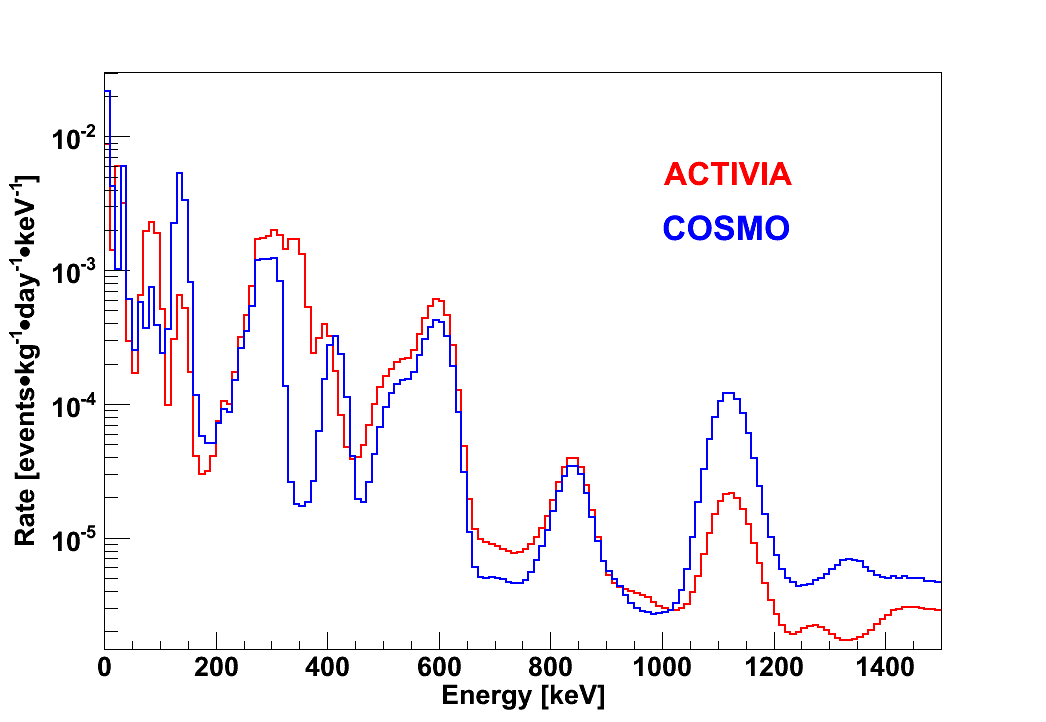
\includegraphics[width=0.475\linewidth]{plots/Cosmogenics/ACTIVIA_COSMO.png}
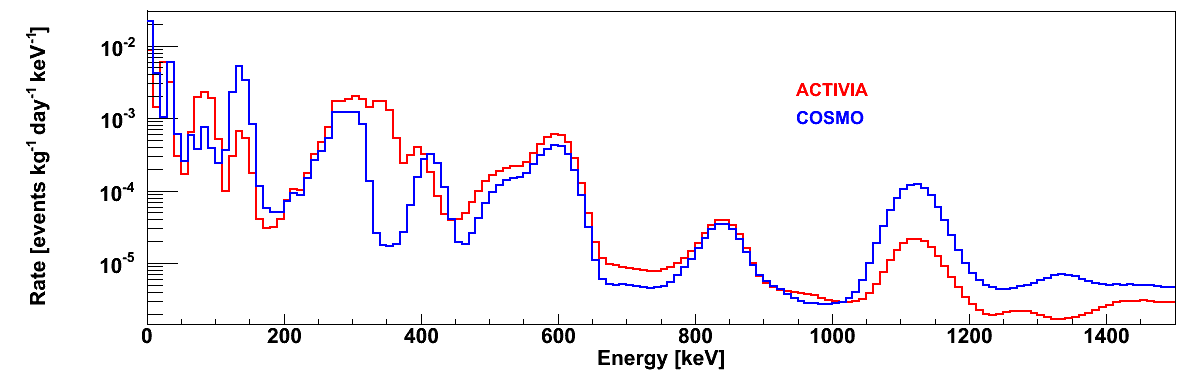
\includegraphics[width=0.75\linewidth]{plots/Cosmogenics/ACTIVIA_COSMO_wide1.png}
%\label{figCosmogenicsSteelDecays_1}}
%\subfigure[]{
%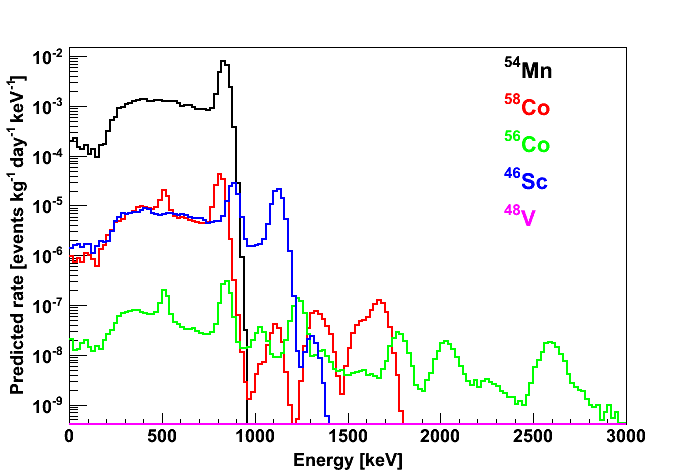
\includegraphics[width=0.475\linewidth]{plots/Cosmogenics/CosmogenicSpectra_LNGSproduction.png}
%\label{figCosmogenicsSteelDecays_2}}
\caption[Predicted energy spectra of the cosmogenic background in the liquid xenon]{Predicted energy spectra of the cosmogenic background in the liquid xenon, for 30~kg fiducial volume. Calculation of the cosmogenic activation has been done with COSMO and ACTIVIA packages, assuming the 1~year activation time and 2~years cooldown. The radioactive decays have been simulated with GEANT4. The predictions with both packages do not agree, and are much higher than the low energy background of $<$10$^{-2}$events$\cdot$kg$^{-1}\cdot$day$^{-1}\cdot$keV$^{-1}$ measured in the commissioning run in Fall 2009 (run07), well explained by the natural radioactivity in the detector and shield materials (see Section~\ref{secDataMCcomparison}).}
\label{figCosmogenicsLXe}
\end{figure}
%\end{floatingfigure}

A Monte Carlo study of the cosmogenic activation in natural xenon target has been performed with the ACTIVIA and COSMO packages mentioned in Section~\ref{secCosmogenicActivationSteel}. The prediction of the production rates (saturation activities) is  presented in Table~\ref{tabCosmogenicsLXe}. 
A similar calculation has been performed for a natural xenon target in Ref.~\cite{CosmogenicProduction_Mei} using the TALYS code~\cite{talys}. The results are compared with ACTIVIA and COSMO in Table.~\ref{tabCosmogenicsLXe}. 
Whereas for some isotopes the production rates calculated with different software packages agree well, for many there is a one order of magnitude disagreement. 
As there are no measurements of cosmogenic activation of the xenon target to be used for a  comparison with the simulations, the predictions are rather unreliable.

The calculation of cosmogenic activation for XENON100 has been performed with ACTIVIA and COSMO, assuming a realistic activation time of 1 year and 2 years of cooldown time underground (two last columns in Table~\ref{tabCosmogenicsLXe}). The decays of all isotopes excluding $^{3}$H (since it is removed during purification~\cite{CosmogenicProduction_Mei}) have been simulated uniformly in the liquid xenon with GEANT4. The results of the simulation are shown in Fig.~\ref{figCosmogenicsLXe}. In the energy region of interest, the predicted background rate is a few events$\cdot$kg$^{-1}\cdot$day$^{-1}\cdot$keV$^{-1}$. These predictions much higher than the measured background level, as shown in Section~\ref{secDataMCcomparison}.

%\begin{table}[!h]
%\centering
%\caption{Cosmogenic activation in the liquid xenon, calculated with different simulation packages.}
%\label{tabCosmogenicsLXe}
%\vspace{0.2cm}
%\begin{tabular}{r | r | c | c | c}
%\hline
%Isotope 		& T$_{1/2}$  	& \multicolumn{3}{c}{Saturation activity [kg$^{-1}\cdot$day$^{-1}$]} \\
%	      		&     		  	& ACTIVIA & COSMO & TALYS \cite{CosmogenicProduction_Mei} \\
%\hline
%$^{3}$H	      		& 12.3~y		& 36.0	& 35.1	& 16.0	\\
%$^{22}$Na 	      	& 2.6~y		& 0.09 	& 0.09	& NA		\\
%$^{45}$Ca 	      	& 165~d		& 0.06 	& 0.05	& NA		\\
%$^{49}$V 	      		& 330~d		& 0.26 	& 0.22	& NA		\\
%$^{54}$Mn 	      	& 312~d		& 0.23 	& 0.20	& NA		\\
%$^{55}$Fe 	      	& 2.7~y		& 0.14 	& 0.12	& NA		\\
%$^{57}$Co 	      	& 271~d		& 0.15 	& 1.69	& NA		\\
%$^{60}$Co 	      	& 5.27~y		& 0.10 	& 0.98	& NA		\\
%$^{65}$Zn 	      	& 244.1~d		& 0.33 	& 3.73	& NA		\\
%$^{68}$Ge 	      	& 270.8~d		& 0.15	& 0.18	& NA		\\
%$^{75}$Se 	      	& 118.5~d		& 0.39 	& 4.17	& NA		\\
%$^{88}$Y 	      		& 106.6~d		& 0.15 	& 1.19	& NA		\\
%$^{93m}$Nb 	      	& 13.6~y		& 0.19 	& 1.09	& NA		\\
%$^{101}$Rh 	      	& 3.3~y		& 1.59 	& 0		& NA		\\
%$^{102}$Rh 	      	& 206~d		& 0.54 	& 0		& NA		\\
%$^{102m}$Rh 	      	& 2.9~y		& 0.54 	& 0		& NA		\\
%$^{110m}$Ag 	      	& 252~d		& 0.08 	& 0		& NA		\\
%$^{109}$Cd 	      	& 1.3~y		& 3.30 	& 0		& 3.2		\\
%$^{113m}$Cd 	      	& 14.0~y		& 0.07 	& 0		& 0.02	\\
%$^{113}$Sn 	      	& 115~d		& 4.59 	& 0.01	& NA		\\
%$^{119m}$Sn 	      	& 250~d		& 0.06 	& 0.09	& 0.02	\\
%$^{125}$Sb 	      	& 2.7~y		& 0.02 	& 1.14	& 0.04	\\
%$^{121m}$Te 	      	& 154~d		& 24.85 	& 16.19	& 11.7	\\
%$^{123m}$Te 	      	& 119.7~d		& 1.23 	& 1.10	& 12.1	\\
%$^{127}$Te 	      	& 109~d		& 1.07 	& 1.06	& 5.0 	\\
%$^{134}$Cs 	      	& 2.1~y		& 0.82 	& 0.83	& NA		\\
%\hline
%\end{tabular}
%\end{table}

